\documentclass{beamer}
\usepackage{amsmath}
\usepackage{amssymb}
\usepackage{animate}
\usepackage{physics}
\usepackage{amsthm}
\usepackage{graphicx}
\usepackage{caption}
\usepackage{subcaption}
\graphicspath{ {./figures/} }
\title{Tomografie a Radonova transformace}
\author{Dominika Hájková, Matyáš Fuksa, Ondřej Kureš}
\institute{Skupina W}
\date{2021}

\begin{document}

\frame{\titlepage}

\begin{frame}
\frametitle{Radonova transformace}
\begin{equation}
\mathcal{R}[f(\vec{x})](\rho, \theta)=_{def} \int_{-\infty}^{+\infty}f(s \vec{\theta}^\perp + \rho \vec{\theta}) \,ds
\end{equation}
\begin{equation}
\mathcal{R}[f(\vec{x})](\rho, \theta)=_{def} \int_{\vec{x}\in \mathbb{R}^2}f(\vec{x})\delta \left(\vec{x}\cdot\vec{\theta} - \rho\right) \,dv_{\vec{x}} 
\end{equation}
Ano, zde je 1. stránka této prezentace. Zde vložíme definici Radonovy transformace (nic moc složitého).
\end{frame}
\begin{frame}
\frametitle{Použití Radonovy transformace - Bod}
Překvapivě, zde je 2. stránka této prezentace. Sem bychom mohli vložit Radonovo transformaci bodu.
\end{frame}
\begin{frame}
\frametitle{Použití Radonovy transformace - Přímka}
\begin{figure}
\begin{columns}
\column{.5\textwidth}
	\animategraphics[loop,autoplay,width=\linewidth]{5}{lines-}{0}{20}
\column{.5\textwidth}
	\animategraphics[loop,autoplay,width=\linewidth]{5}{sino-}{0}{20}
	 \label{fig:sub3}
\end{columns}
\end{figure}
\end{frame}
\begin{frame}
\frametitle{Použití Radonovy transformace - Přímky v obraze}
\begin{figure}
\begin{columns}
\column{.5\textwidth}
	  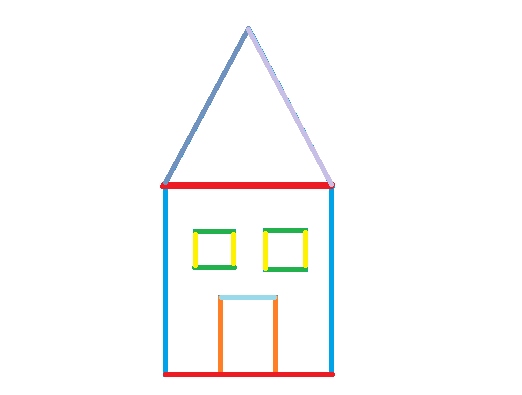
\includegraphics[width=\linewidth]{house.png}
\column{.5\textwidth}
	  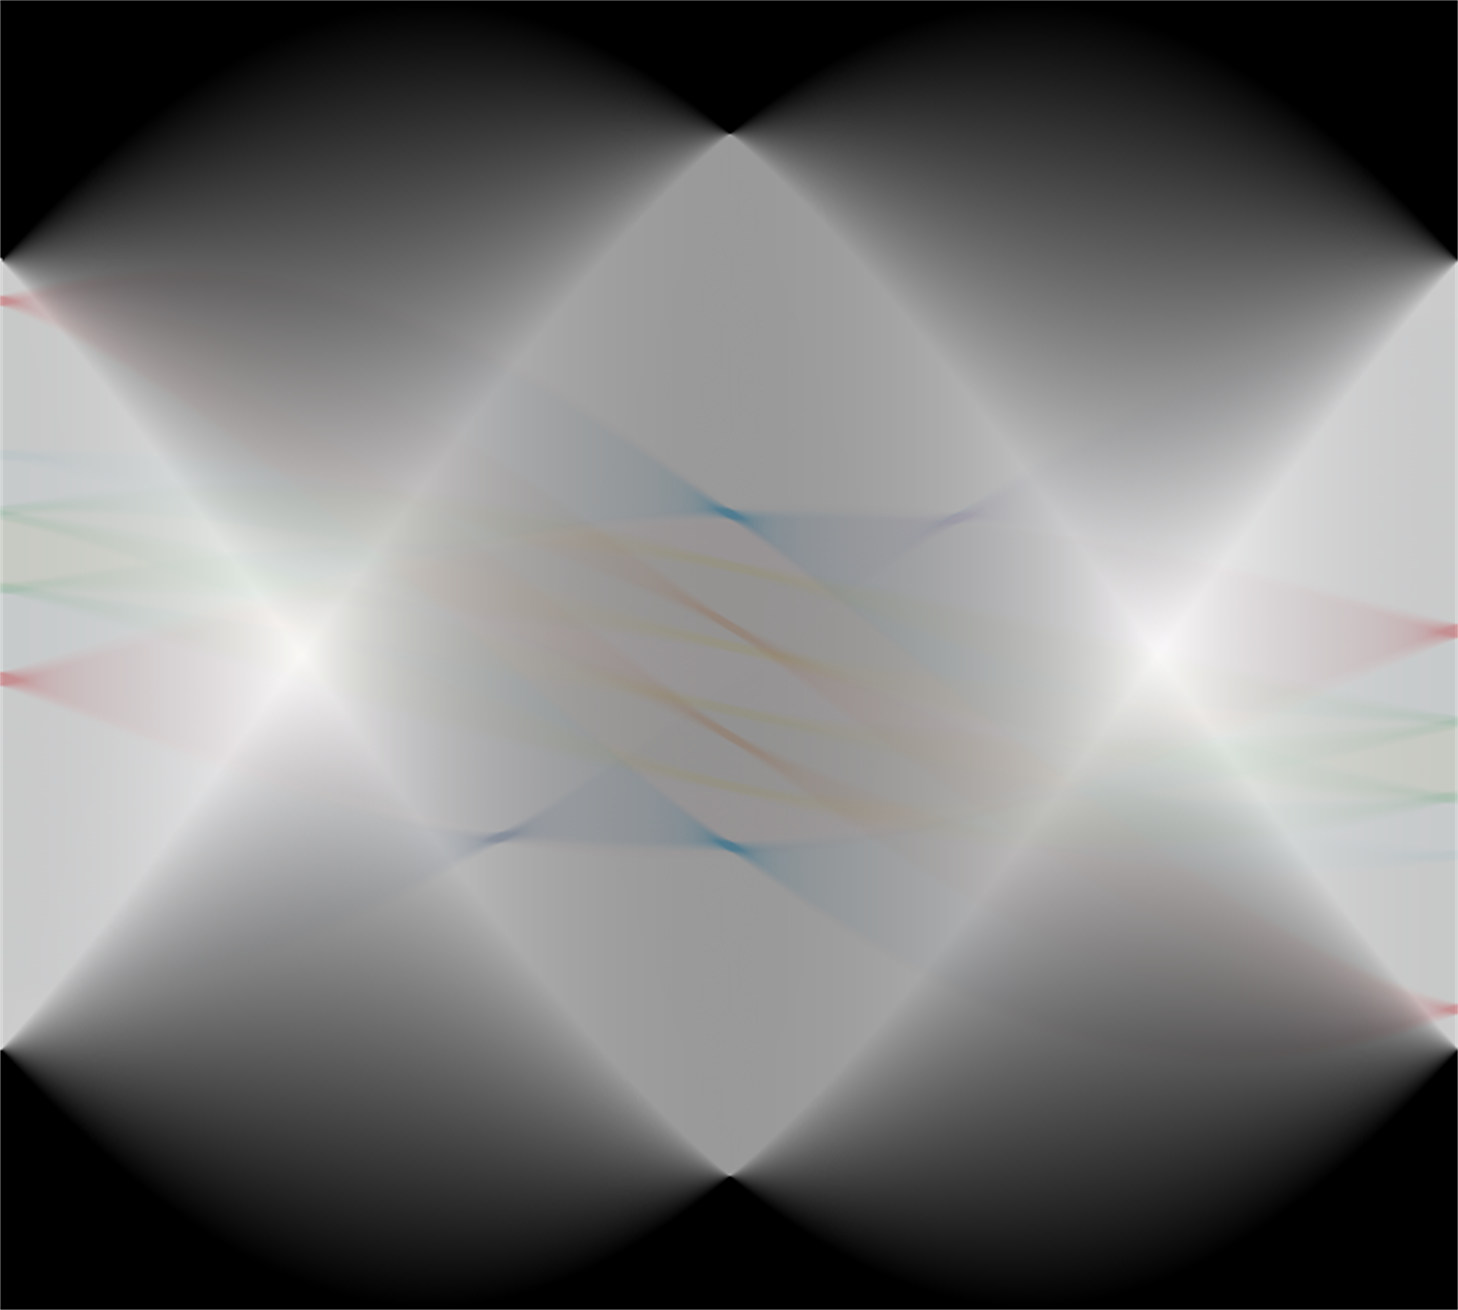
\includegraphics[width=\linewidth]{sinohouse.png}
	 \label{fig:sub4}
\end{columns}
\end{figure}
Podle barevného rozlišení lze určit:
\begin{itemize}
\item Svislé přímky okolo středu
\item Vodorovné vycházejí z okrajů
\end{itemize}
\end{frame}
\begin{frame}
\frametitle{Inverzní Radonova transformace}
\begin{itemize}
\item Pomocí Fourierovy transformace - přes (jednodimenziální) vrstvu - nepoužíváno v praxi
\item Taktéž přes Fourierovu transformaci:
\end{itemize}
\begin{equation}
f(\vec{x})=  \int_{\theta=0}^{\pi}
	\left\lbrace
		\mathcal{H}_{\rho \to \xi}
			\left[\frac{\partial}{\partial\rho}
				\left(\mathcal{R}[f(\vec{x})](\rho,\theta)
				\right)
			\right]
		(\xi,\theta)
	\right\rbrace
	_{\xi = \vec{x}\cdot\vec{\theta}}
	\,d\theta
\end{equation}
Kde $\mathcal{H}$ představuje Hilbertovu transformaci. Výsledný vzorec v praxi též nepoužíván kvůli náročnosti výpočtu.
\begin{itemize}
\item V praxi aproximace: metoda filtrované zpězné projekce
\end{itemize}
 \begin{equation}
   	\mathcal{F}^{-1}_{\nu \to \xi}\left[|{\nu}|\mathcal{F}_{\nu \to \xi}\left[\mathcal{R}f\right]\right]
	\approx
    \sqrt{\frac{2}{\pi}}
    \left(W\frac{\sin\left(\xi W\right)}{\xi}
      +\frac{\cos \left( \xi W \right)}{\xi ^2}-\frac{1}{\xi^2}\right)*\mathcal{R}f	
\end{equation}
\end{frame}

\begin{frame}
\frametitle{Co snědla Vítkova dcerka?}

\begin{figure}
\centering
\begin{subfigure}{.5\textwidth}
  \centering
  
\includegraphics[width=.8\linewidth]{secret-radon.pdf}
  \label{fig:sub1}
\end{subfigure}%
\begin{subfigure}{.5\textwidth}
  \centering
  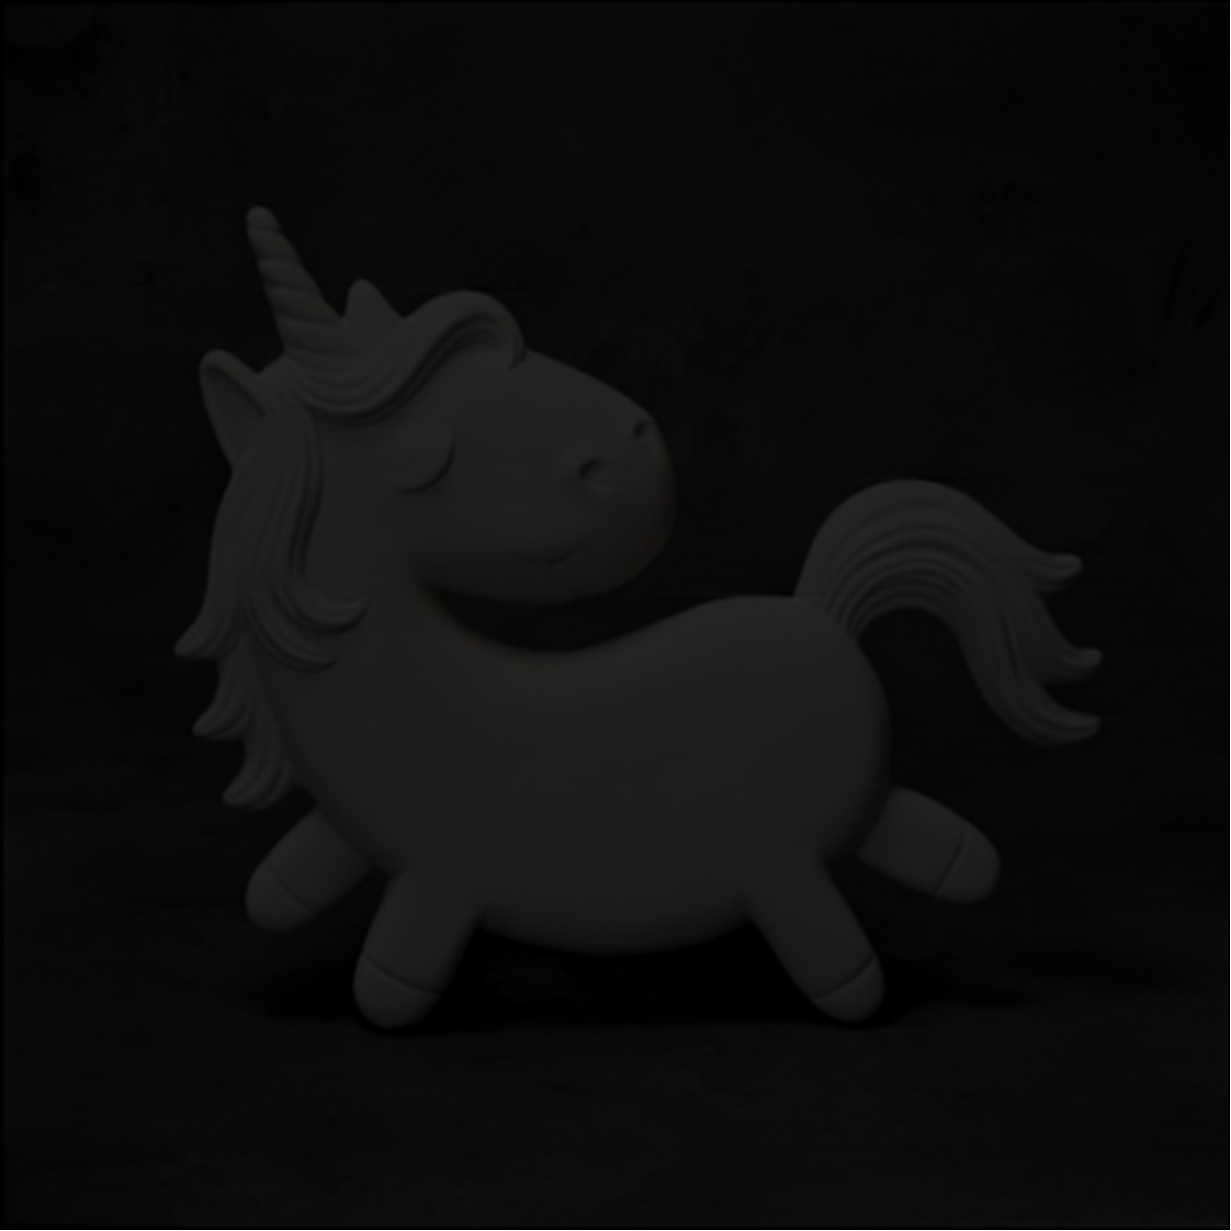
\includegraphics[width=.8\linewidth]{unicorn.pdf}
  \label{fig:sub2}
\end{subfigure}
\caption{Skrytý obrázek a odhalený obrázek}
\label{fig:test}
\end{figure}

\end{frame}
\begin{frame}
\begin{center}
\begin{huge}
Děkujeme za pozornost
\end{huge}

\end{center}

\end{frame}
\end{document}